\newpage
\section{USE CASE CHI TIẾT VÀ SƠ ĐỒ HOẠT ĐỘNG, SƠ ĐỒ LỚP CỦA HỆ THỐNG}
\subsection{Sơ đồ Use Case của hệ thống}

\begin{figure}[H]
    \centering
    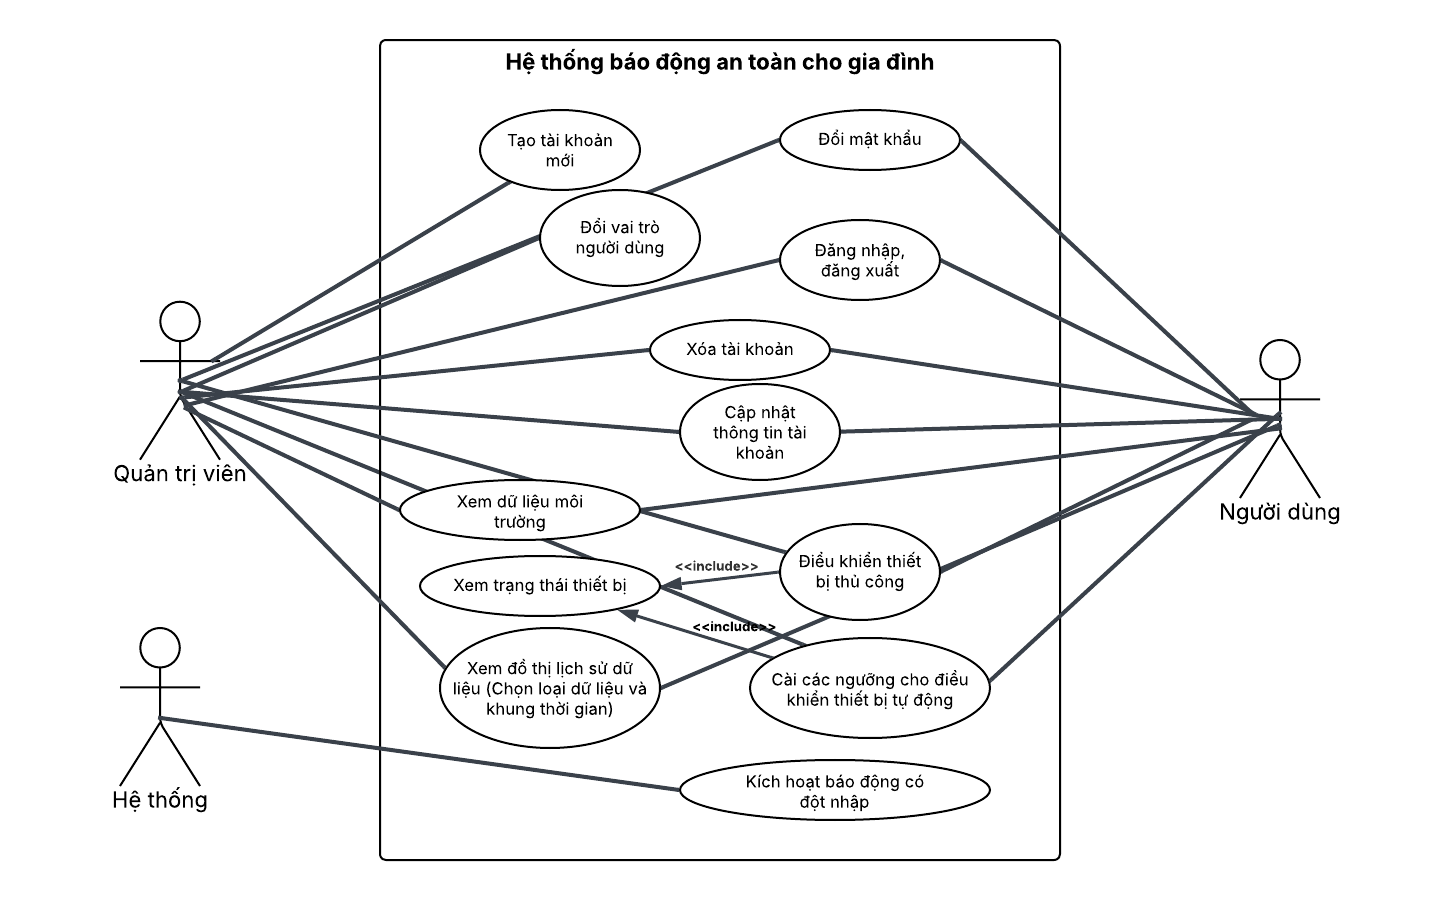
\includegraphics[width=\textwidth]{figures/usecase_diagram.png}
    \caption{Sơ đồ Use Case của hệ thống}
    \label{fig:usecase_diagram}
\end{figure}

\subsection{Đặc tả Use Case của hệ thống}
\begin{longtable}{|p{0.2\textwidth}|p{0.8\textwidth}|}
    \hline
    \textbf{Use Case}         & Thiết lập ngưỡng cho điều khiển tự động                                                                                                     \\
    \hline
    \textbf{Actors}           & Người dùng, admin                                                                                                                           \\
    \hline
    \textbf{Descriptions}     & Cho phép người dùng thiết lập ngưỡng (slider) cho các cảm biến như nhiệt độ, ánh sáng, khoảng cách để hệ thống điều khiển thiết bị tự động. \\
    \hline
    \textbf{Precondition}     &
    - Người dùng đã đăng nhập thành công. \newline
    - Cảm biến đang hoạt động bình thường.                                                                                                                                  \\
    \hline
    \textbf{Normal flow}      &
    1. Người dùng mở giao diện cài đặt tự động. \newline
    2. Hệ thống hiển thị các slider ngưỡng cho từng cảm biến. \newline
    3. Người dùng kéo slider để điều chỉnh ngưỡng phù hợp. \newline
    4. Hệ thống lưu các ngưỡng vào cơ sở dữ liệu. \newline
    5. Thông báo thiết lập thành công.                                                                                                                                      \\
    \hline
    \textbf{Alternative flow} &
    \textbf{Alternative 1:} \newline
    - Nếu người dùng nhập giá trị vượt mức cho phép, hệ thống hiển thị cảnh báo và không cho lưu.                                                                           \\
    \hline
    \textbf{Exceptions}       &
    \textbf{Exception 1:} \newline
    - Lỗi kết nối cơ sở dữ liệu khiến không thể lưu thiết lập.                                                                                                              \\
    \hline
    \caption{Use Case 1: Thiết lập ngưỡng tự động}
    \label{tab:usecase1}
\end{longtable}


\begin{longtable}{|p{0.2\textwidth}|p{0.8\textwidth}|}
    \hline
    \textbf{Use Case}         & Điều khiển thủ công thiết bị                                                                  \\
    \hline
    \textbf{Actors}           & Người dùng, admin                                                                             \\
    \hline
    \textbf{Descriptions}     & Người dùng có thể điều khiển bật/tắt thiết bị như quạt, đèn, khóa cửa thủ công qua giao diện. \\
    \hline
    \textbf{Precondition}     &
    - Người dùng đã đăng nhập. \newline
    - Thiết bị được thêm vào hệ thống và đang hoạt động.                                                                      \\
    \hline
    \textbf{Normal flow}      &
    1. Người dùng chọn phòng và thiết bị muốn điều khiển. \newline
    2. Giao diện hiển thị trạng thái hiện tại của thiết bị. \newline
    3. Người dùng chọn hành động (bật/tắt). \newline
    4. Hệ thống gửi lệnh điều khiển đến phần cứng. \newline
    5. Giao diện cập nhật trạng thái mới.                                                                                     \\
    \hline
    \textbf{Alternative flow} &
    \textbf{Alternative 1:} \newline
    - Nếu thiết bị không phản hồi, hệ thống hiển thị thông báo lỗi.                                                           \\
    \hline
    \textbf{Exceptions}       &
    \textbf{Exception 1:} \newline
    - Lỗi giao tiếp phần cứng hoặc thiết bị ngoại tuyến.                                                                      \\
    \hline
    \caption{Use Case 2: Điều khiển thủ công thiết bị}
    \label{tab:usecase2}
\end{longtable}


\begin{longtable}{|p{0.2\textwidth}|p{0.8\textwidth}|}
    \hline
    \textbf{Use Case}         & Kích hoạt báo động                                                                                                              \\
    \hline
    \textbf{Actors}           & Hệ thống                                                                                                                        \\
    \hline
    \textbf{Descriptions}     & Khi giá trị cảm biến vượt ngưỡng cho phép (khoảng cách gần, nhiệt độ cao), hệ thống tự động bật báo động trên web và phần cứng. \\
    \hline
    \textbf{Precondition}     &
    - Thiết lập ngưỡng đã được cấu hình. \newline
    - Thiết bị và cảm biến đang hoạt động.                                                                                                                      \\
    \hline
    \textbf{Normal flow}      &
    1. Cảm biến gửi dữ liệu mới. \newline
    2. Hệ thống kiểm tra ngưỡng. \newline
    3. Nếu vượt ngưỡng, hệ thống: \newline
    \quad - Phát âm thanh cảnh báo trên web. \newline
    \quad - Chớp đèn LED cảnh báo phần cứng. \newline
    \quad - Khóa cửa (nếu là cảnh báo xâm nhập). \newline
    4. Giao diện web hiển thị chỉ số màu đỏ và in đậm.                                                                                                          \\
    \hline
    \textbf{Alternative flow} &
    \textbf{Alternative 1:} \newline
    - Nếu mức chỉ vượt nhẹ, chỉ hiển thị cảnh báo nhẹ, không kích hoạt toàn bộ hệ thống.                                                                        \\
    \hline
    \textbf{Exceptions}       &
    \textbf{Exception 1:} \newline
    - Nếu không thể điều khiển thiết bị vật lý, hệ thống chỉ cảnh báo trên web.                                                                                 \\
    \hline
    \caption{Use Case 3: Kích hoạt báo động}
    \label{tab:usecase3}
\end{longtable}


\begin{longtable}{|p{0.2\textwidth}|p{0.8\textwidth}|}
    \hline
    \textbf{Use Case}         & Xem Dashboard dữ liệu cảm biến                                                                      \\
    \hline
    \textbf{Actors}           & Người dùng                                                                                          \\
    \hline
    \textbf{Descriptions}     & Hệ thống hiển thị biểu đồ dữ liệu cảm biến theo thời gian thực hoặc theo khoảng thời gian chọn lọc. \\
    \hline
    \textbf{Precondition}     &
    - Dữ liệu cảm biến đang được ghi nhận và lưu. \newline
    - Người dùng đã đăng nhập.                                                                                                      \\
    \hline
    \textbf{Normal flow}      &
    1. Người dùng vào giao diện dashboard. \newline
    2. Chọn loại dữ liệu muốn xem (nhiệt độ, độ ẩm...). \newline
    3. Chọn thời gian: 1 phút, 5 phút, hoặc tùy chỉnh. \newline
    4. Biểu đồ cập nhật theo thời gian thực (cập nhật mỗi 2 giây). \newline
    5. Hiển thị thông tin rõ ràng, các ngưỡng vượt mức được in đậm.                                                                 \\
    \hline
    \textbf{Alternative flow} &
    \textbf{Alternative 1:} \newline
    - Nếu không có dữ liệu trong khoảng thời gian chọn, hiển thị “Không có dữ liệu”.                                                \\
    \hline
    \textbf{Exceptions}       &
    \textbf{Exception 1:} \newline
    - Lỗi truy vấn dữ liệu từ cơ sở dữ liệu.                                                                                        \\
    \hline
    \caption{Use Case 4: Xem Dashboard dữ liệu cảm biến}
    \label{tab:usecase4}
\end{longtable}


\begin{longtable}{|p{0.2\textwidth}|p{0.8\textwidth}|}
    \hline
    \textbf{Use Case}         & Quản lý tài khoản người dùng                                                       \\
    \hline
    \textbf{Actors}           & Admin                                                                              \\
    \hline
    \textbf{Descriptions}     & Admin có thể chỉnh sửa, xóa tài khoản người dùng, hoặc thêm mới tài khoản nếu cần. \\
    \hline
    \textbf{Precondition}     &
    - Admin đã đăng nhập hệ thống.                                                                                 \\
    \hline
    \textbf{Normal flow}      &
    1. Admin truy cập giao diện quản lý tài khoản. \newline
    2. Xem danh sách tài khoản hiện tại. \newline
    3. Chọn thao tác: sửa, xóa, hoặc thêm mới. \newline
    4. Thực hiện thao tác và lưu thay đổi. \newline
    5. Hệ thống hiển thị thông báo thành công.                                                                     \\
    \hline
    \textbf{Alternative flow} &
    \textbf{Alternative 1:} \newline
    - Nếu người dùng không có quyền admin, giao diện không hiển thị tính năng này.                                 \\
    \hline
    \textbf{Exceptions}       &
    \textbf{Exception 1:} \newline
    - Lỗi kết nối cơ sở dữ liệu gây thất bại thao tác.                                                             \\
    \hline
    \caption{Use Case 5: Quản lý tài khoản người dùng}
    \label{tab:usecase5}
\end{longtable}


\subsection{Sơ đồ hoạt động của hệ thống}

\begin{figure}[H]
    \centering
    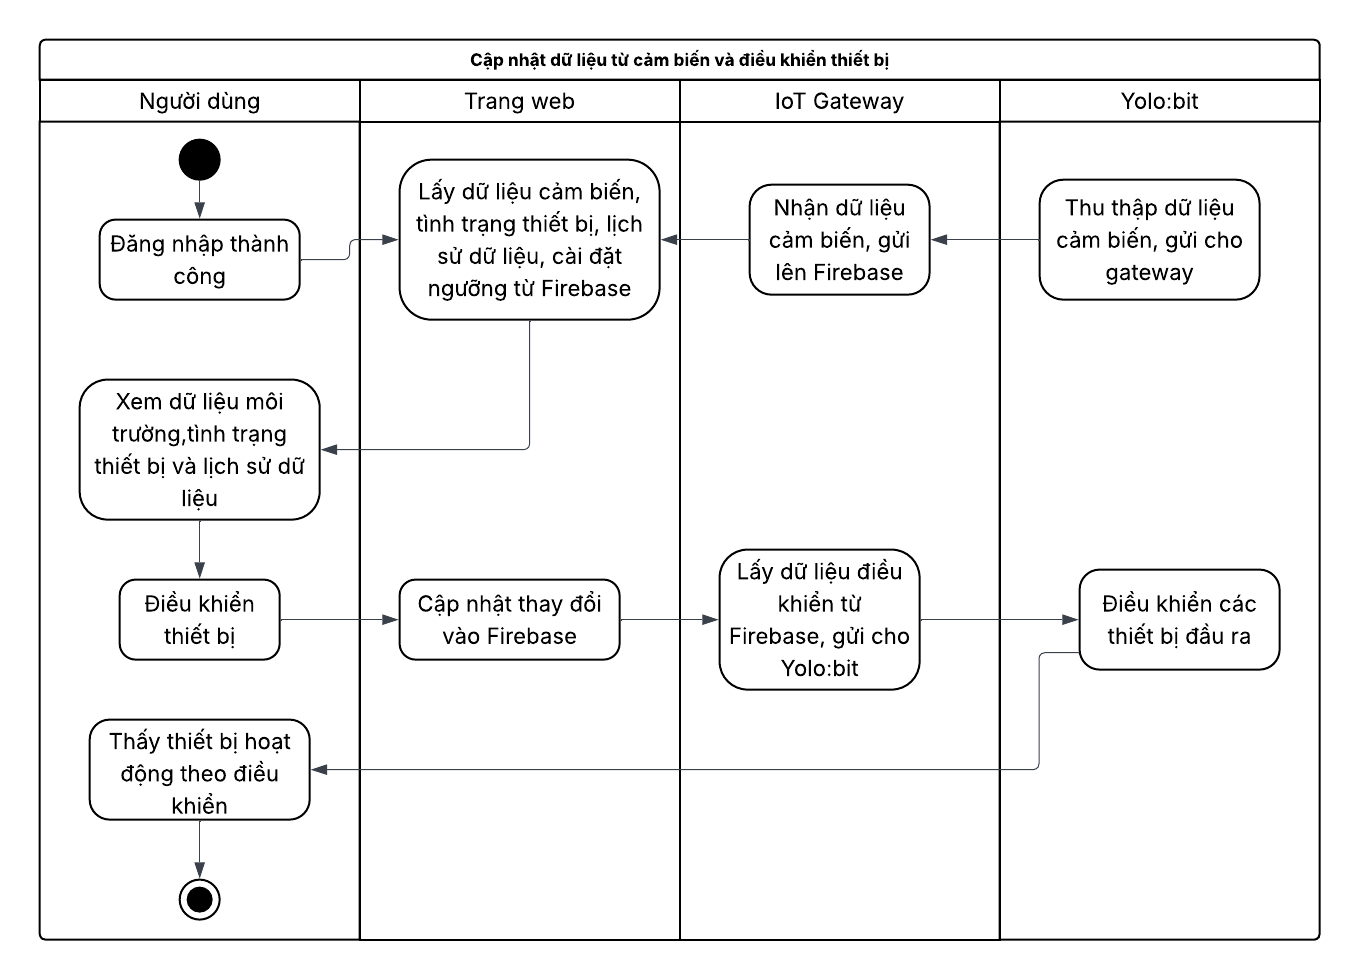
\includegraphics[width=0.8\textwidth]{figures/activity_1.png}
    \caption{Sơ đồ hoạt động cho cập nhật dữ liệu từ cảm biến và điều khiển thiết bị}
    \label{fig:activity_1}
\end{figure}

\begin{figure}[H]
    \centering
    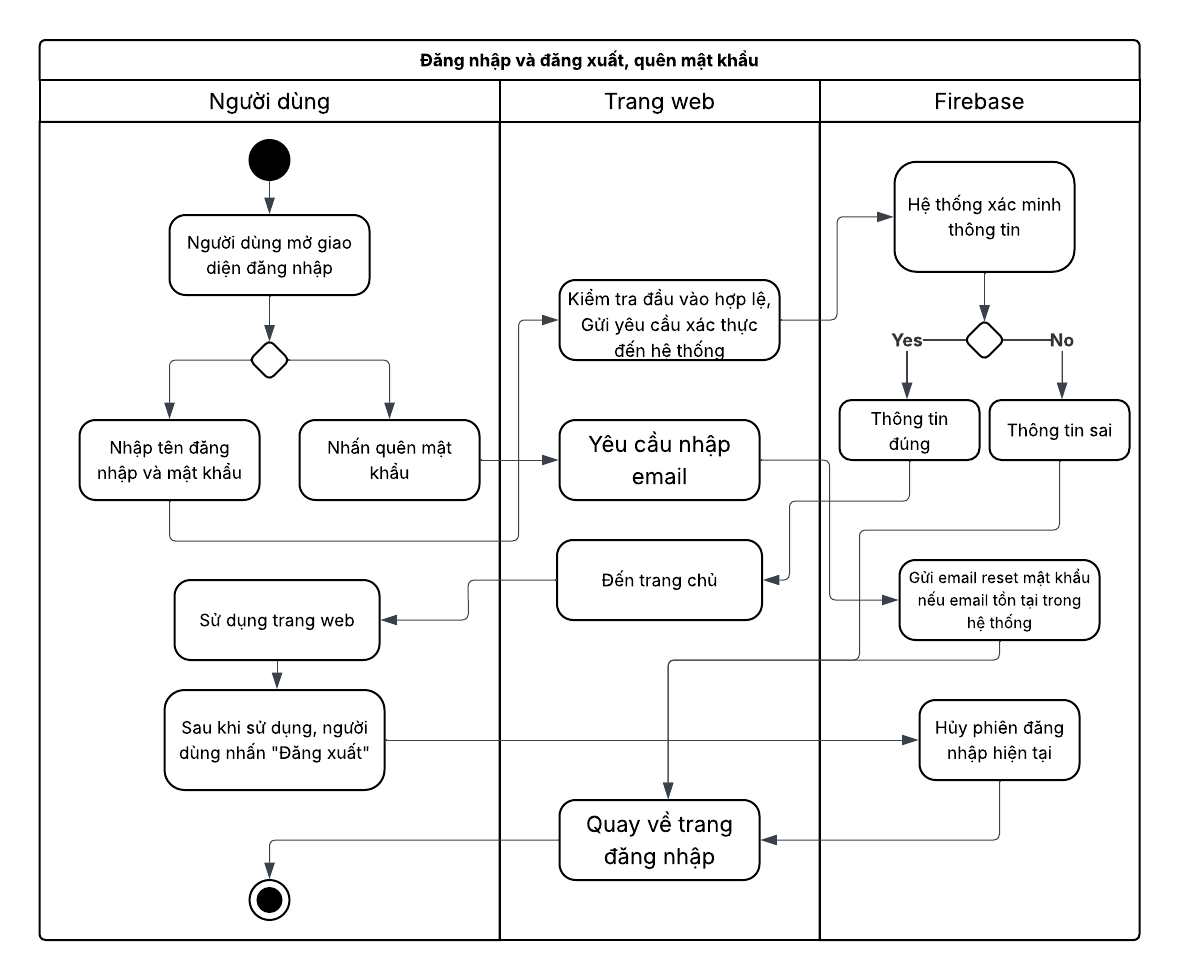
\includegraphics[width=0.8\textwidth]{figures/activity_2.png}
    \caption{Sơ đồ hoạt động cho đăng nhập và đăng xuất, quên mật khẩu}
    \label{fig:activity_2}
\end{figure}

\begin{figure}[H]
    \centering
    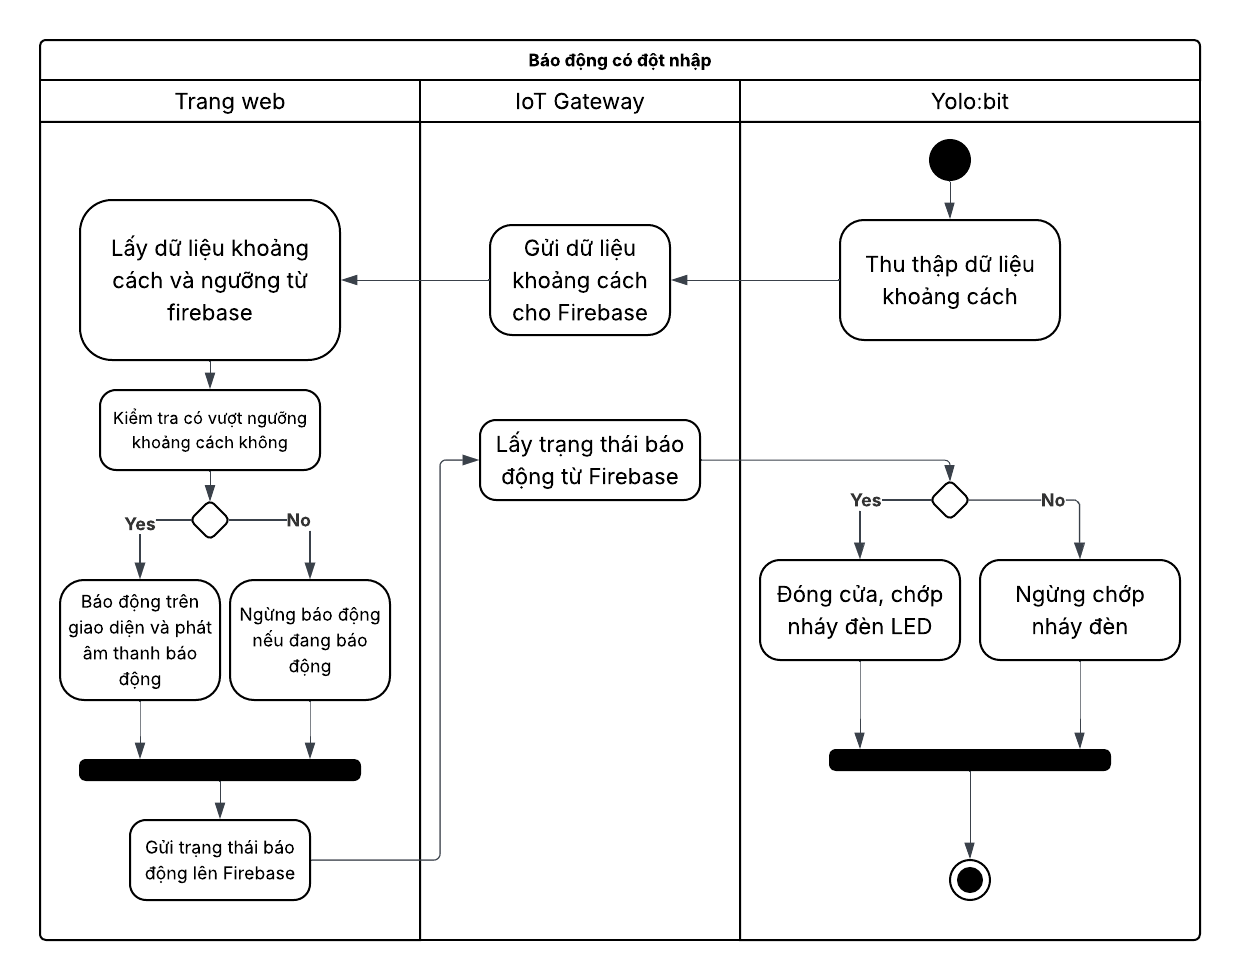
\includegraphics[width=0.8\textwidth]{figures/activity_3.png}
    \caption{Sơ đồ hoạt động cho báo động có đột nhập}
    \label{fig:activity_3}
\end{figure}

\begin{figure}[H]
    \centering
    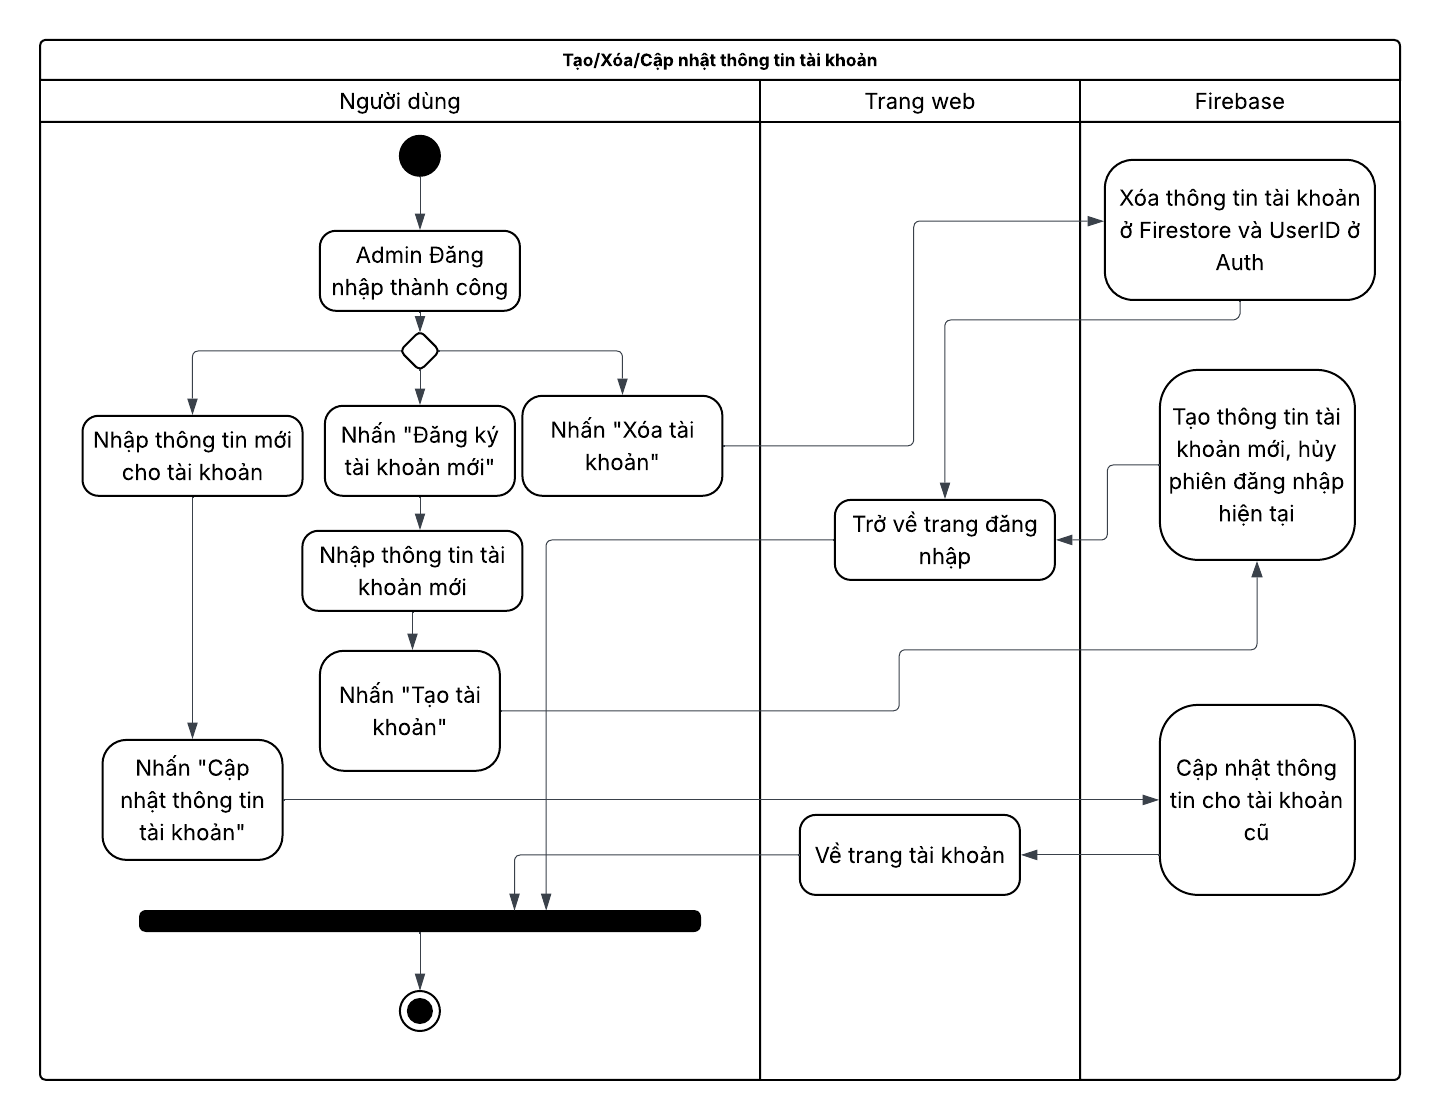
\includegraphics[width=0.8\textwidth]{figures/activity_4.png}
    \caption{Sơ đồ hoạt động cho tạo-xóa-cập nhật thông tin tài khoản}
    \label{fig:activity_4}
\end{figure}


\subsection{Sơ đồ lớp của hệ thống}

Các lớp quan trọng bao gồm: \textbf{Người dùng}, \textbf{Cảm biến}, \textbf{Ngưỡng}, \textbf{Dữ liệu cảm biến}, \textbf{Cảnh báo}. Trong đó, \textbf{Người dùng} là đối tượng trung tâm, có thể quản lý các cảm biến, thực hiện thay đổi ngưỡng, theo dõi dữ liệu.

Mỗi \textbf{Cảm biến} gắn với một giá trị \textbf{Ngưỡng}, được sử dụng để xác định khi nào dữ liệu vượt giới hạn an toàn. Khi cảm biến hoạt động sẽ liên tục tạo ra \textbf{Dữ liệu cảm biến}, bao gồm giá trị của cảm biến đó và thời gian ghi nhận. Nếu dữ liệu gần đây nhất vượt ngưỡng, hệ thống sẽ tạo một \textbf{Cảnh báo} và gửi đến người dùng để xử lý kịp thời. Mỗi cảm biến có kiểu, vị trí và trạng thái. Phương thức \texttt{readData()} trả về dữ liệu cảm biến, trong khi \texttt{checkThreshold()} kiểm tra ngưỡng và \texttt{triggerAlert()} tạo cảnh báo nếu vượt quá ngưỡng.

Lớp \textbf{Người dùng} đại diện cho cá nhân quản lý hệ thống, có các thuộc tính như \texttt{name}, \texttt{email} và \texttt{password}.

Lớp \textbf{Ngưỡng} định nghĩa giới hạn cho từng cảm biến. Bao gồm giá trị tối thiểu và tối đa, và phương thức \texttt{isWithinRange()} để kiểm tra một giá trị có nằm trong khoảng cho phép hay không.

Lớp \textbf{Dữ liệu cảm biến} lưu lại thông tin được thu thập, bao gồm giá trị, thời gian và trạng thái. Mỗi bản ghi được tạo ra bởi cảm biến và được lưu trữ bằng phương thức \texttt{store()}.

Lớp \textbf{Cảnh báo} được tạo ra khi dữ liệu cảm biến vượt quá ngưỡng. Nó ghi nhận loại cảnh báo, thời gian và trạng thái, đồng thời có thể gửi thông báo cho người dùng (\texttt{notifyUser()}) và ghi nhật ký (\texttt{logAlert()}).

Mối quan hệ giữa các lớp chủ yếu là quan hệ một-nhiều (\textit{one-to-many}), chẳng hạn như một người dùng quản lý nhiều cảm biến, một cảm biến có thể tạo ra nhiều dữ liệu hoặc cảnh báo.

\begin{figure}[H]
    \centering
    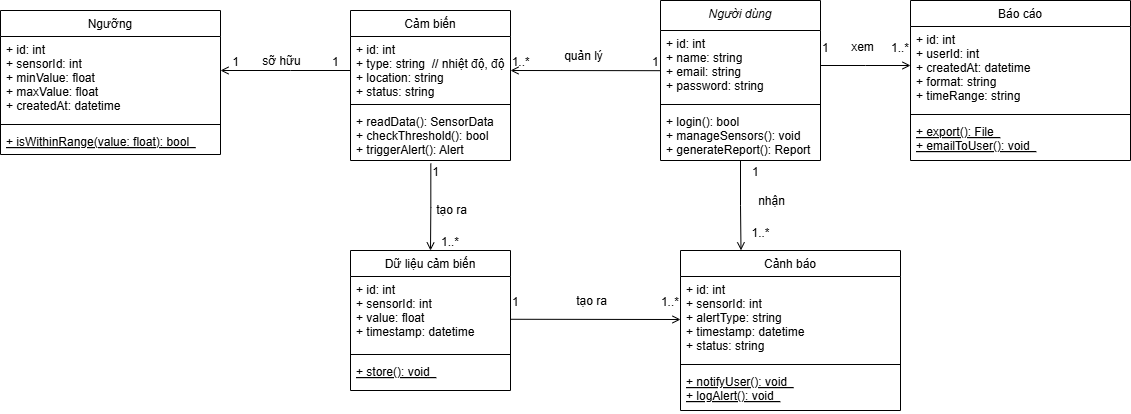
\includegraphics[width=\textwidth]{figures/class_diagram.png}
    \caption{Sơ đồ lớp của hệ thống}
    \label{fig:class_diagram}
\end{figure}